% Шаблон для Ed-era.com
\documentclass[a4paper,12pt]{article}
\usepackage{edera}
\usepackage[margin=1.in]{geometry} % отступы
\usepackage{wrapfig}
\usepackage{hyperref} 
\usepackage{tabularx}
\usepackage{multicol} % Несколько колонок
\usetikzlibrary{arrows}
\definecolor{cqcqcq}{rgb}{0.7529411764705882,0.7529411764705882,0.7529411764705882}
\usepackage{mathtext} 
%\usepackage[usenames,dvipsnames,svgnames,table,rgb]{xcolor}
\hypersetup{				% Гиперссылки
	unicode=true,           % русские буквы в раздела PDF
	pdftitle={Заголовок},   % Заголовок
	pdfauthor={Автор},      % Автор
	pdfsubject={Тема},      % Тема
	pdfcreator={Создатель}, % Создатель
	pdfproducer={Производитель}, % Производитель
	pdfkeywords={keyword1} {key2} {key3}, % Ключевые слова
	colorlinks=true,       	% false: ссылки в рамках; true: цветные ссылки
	linkcolor=black,          % внутренние ссылки
	citecolor=green,        % на библиографию
	filecolor=magenta,      % на файлы
	%	urlcolor=EdEraOrange          % на URL
}


\newenvironment{eeprob}[3]
{
\begin{table}[!h]
\setlength{\arrayrulewidth}{1.pt}
\arrayrulecolor[HTML]{EFA72D}
\begin{tabularx}{\textwidth}{|c X}
\cellcolor[HTML]{EFA72D} \color{white}\textbf{Задача #1}& \textbf{#2} \\ 
& 
\end{tabularx}
%\caption{Заголовок мог быть и здесь}
\end{table}
\vspace{-1.2cm}
\begin{table}[!h]
\setlength{\arrayrulewidth}{1.pt}
\arrayrulecolor[HTML]{EFA72D}
\begin{tabularx}{\textwidth}{|X}
#3 \\ 
\end{tabularx}
\end{table}
}
{\arrayrulecolor{black}}

\usepackage{mathtext} 
% % % % % % % % % % % % % % % % % % % % % % % % % % % % % % % % % % % %
\usepackage{fancyhdr} % Колонтитулы
\pagestyle{fancy}
%\renewcommand{\headrulewidth}{0mm}  % Толщина линейки, отчеркивающей верхний колонтитул
\lfoot{ }
\rhead{\href{Ed-era.com}{\textcolor{EdErablue}{Ed}\textcolor{EdEraorange}{Era}} \,\, Філіпов Ілля }
\lhead{"Ф.\MakeUppercase{\romannumeral1} :  Двовимірна кінематика 2/2
"}
% % % % % % % % % % % % % % % % % % % % % % % % % % % % % % % % % % % % %
\title{\textbf{Фізика} \textbf{\MakeUppercase{\romannumeral1}}\\
	\textbf{Механіка}\\
	\textbf{Концепція сили 2/3}}
\date{}
\author{}

\begin{document}
\thispagestyle{empty}
\textcolor{white}{.}
\vfill
\begin{center} 
\vspace{-6cm} 

\includegraphics[width = .85\textwidth]{EdEra.pdf}
\end{center}
\vfill
\newpage
\maketitle
\vspace{3cm}
\tableofcontents
\newpage


\tikzstyle{abstract}=[rectangle,rounded corners,draw = EdErablue,top color = white, bottom color=EdEraorange,very thick, inner sep=0.3em, text centered, anchor=north, text=EdErablue, text width=3cm]
\tikzstyle{empty}=[rectangle,rounded corners,,very thick, inner sep=0.3em, text centered, anchor=north, text=black, text width=3cm]
\tikzstyle{line}=[-, thick, color = EdErablue]

% % % % % % % % % % % % % % % % % % % % % % % % % % % % % % % % % % %
\newpage
% % % % % % % % % % % % Тут почінається конспект % % % % % % % % % % 	

\section{Реакція опори та підвісу}
\textbf{\textcolor{EdErablue}{Перед вами дві ситуації $\rightarrow$}}
\begin{center}
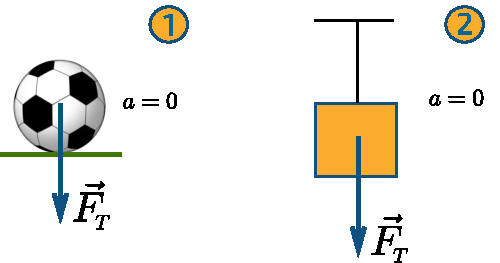
\includegraphics[scale=0.9]{P1}
\end{center}
В обох ситуаціях на тіло діє сила тяжіння. З іншого боку в обох ситуаціях прискорення $a = 0$. За другим законом Ньютона нульове прискорення може бути при умові, що рівнодійна сили дорівнює нулю. Силу тяжіння урівноважує так звана \textcolor{EdErablue}{\textbf{сила реакції опори або підвісу}}. 

\eoz{\begin{itemize} \item[\textcolor{EdErablue}{\textbf{1.}}] \textbf{\textcolor{EdErablue}{Сила реакції опори $\vec{N}$}} - сила, що діє на тіло зі сторони опори (поверхні). Напрямлена перпендикулярно до поверхні, тому її також називають \textbf{нормальною силою}.  \item[\textcolor{EdErablue}{\textbf{2.}}]\textcolor{EdErablue}{\textbf{Сила натягу нитки $\vec{T}$}} – сила, що діє на тіло з боку нитки. Напрямлена вздовж неї. \end{itemize} У двох зображених випадках ці сили виникають згідно з \textbf{третім законом \,\,\,\,Ньютона}. Внаслідок сили тяжіння тіло діє на опору (підвіс), які у свою чергу діють на тіло з такою самою силою, але у протилежному напрямку.}
Зображувати дію усіх сил на центр тіла можна у випадку розгляду тіл, як матеріальних точок. В цьому курсі виключення будуть вказані. 
\begin{center}
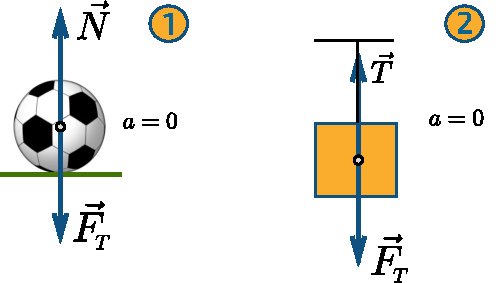
\includegraphics[scale=0.9]{P2}
\end{center}
\newpage
\subsection{Сила реакції опори та вага}
\textcolor{EdErablue}{\textbf{Важливо}} пригадати формулювання третього закону Ньютона: \begin{center}
\textit{« Тіла діють одне на одне із силами, спрямованими вздовж однієї прямої, рівними за модулем і протилежними за напрямком. »} $$\boxed{\vec{F}_A = - \vec{F}_R}$$
\end{center}
$F_A$ - дія першого тіла на друге; $F_R$ - дія другого тіла на перше\\

У розглянутих нами випадках сила тяжіння і сила реакції опори – сили, що діють \textbf{на} тіло. Отже, вони не є силами з визначення третього закону Ньютона. Сила реакції опори за третім законом Ньютона дорівнює силі, з якою тіло діє на опору або підвіс. Ця сила називається \textcolor{EdErablue}{\textbf{вагою}}.

\eoz{\textbf{Вага $\vec{P}$} – сила, з якою тіло діє на горизонтальну опору або вертикальний підвіс. За третім законом Ньютона дорівнює по модулю \textbf{силі реакції опори} $\vec{N}$. }

\hspace{-0.8cm} Вимірюється вага за допомогою \textcolor{EdErablue}{\textbf{вагів або терезів}}. Сучасні ваги на своєму табло показують масу тіла. Насправді вони вимірюють \textbf{силу}, з якою тіло тисне на них – вагу, а потім здійснюється перерахунок у масу і виводиться на екран. У випадку, коли ваги нерухомо стоять на землі вага дорівнює силі тяжіння $P = mg$.\\
\newline
\ealgorithm{Отримання ваги в задачах}{Вага за третім законом Ньютона дорівнює за модулем силі реакції опори або підвіса. \begin{center}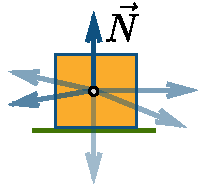
\includegraphics[scale=0.8]{P3}\end{center}\begin{itemize}\item[1.] За другим законом Ньютона рівнодійна сил дорівнює масі тіла помноженій на прискорення: $$\vec{F_1} + \vec{F_2} + ... + \vec{F_N} = m\vec{a}$$ \item[2.] Розв'язуючи це рівняння, наприклад, за допомогою розкладання на проекції, виражаємо силу реакції опори або підвіса (в залежності від задачі) $$\vec{N}/\vec{T}$$ \item[3.] За третім законом Ньютона: $$\vec{P} = -\vec{N}$$\end{itemize}}

\newpage
\subsection{Приклади}
Зараз ми розглянемо кілька розповсюджених прикладів на знаходження ваги $\vec{P}$.
\subsubsection{Рух у ліфті}
\begin{center}
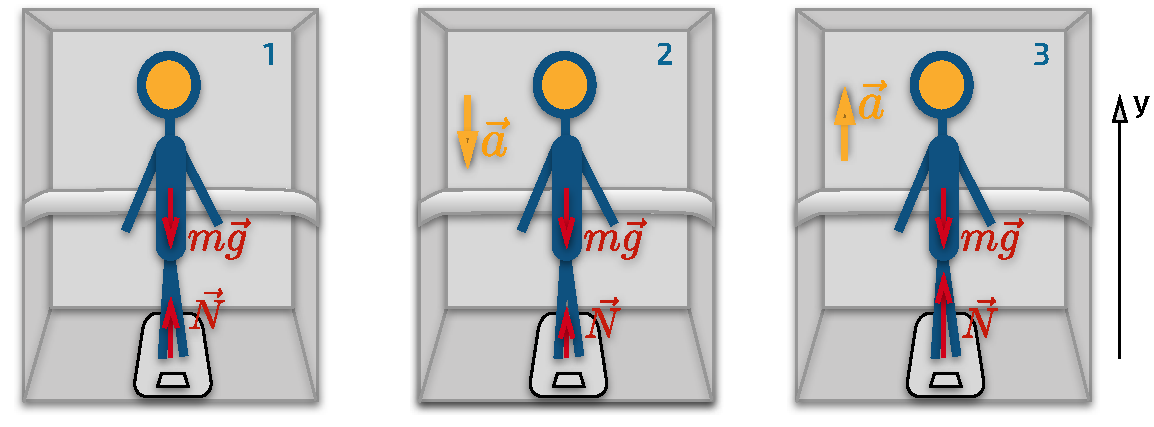
\includegraphics[scale=0.7]{P5}
\end{center}
Розглядаємо три випадки руху в ліфті: рівномірний або стан спокою, рівноприскорений (вгору), рівноприскорений (вниз). Оцінимо, як будуть відрізнятися покази вагів. \\ \newline На тіло діє всього дві сили: сила тяжіння $\vec{F}_{\text{т}} = m\vec{g}$ та сила реакції опори $\vec{N}$.
\\ \newline Другий закон Ньютона: $$\vec{N} + m\vec{g} = m\vec{a}$$
\begin{itemize}
\item[\textcolor{EdErablue}{\textbf{1.}}] \textcolor{EdErablue}{ \textbf{Ліфт у стані спокою або рухається с постійною швидкістю $\boxed{a = 0}$}}\\ Другий закон Ньютона в проекції на y: $$N - mg = 0\,\,\Rightarrow\,\,N = mg$$ Третій закон Ньютона: $$P = N = mg$$
\item[\textcolor{EdErablue}{\textbf{2.}}] \textcolor{EdErablue}{ \textbf{Ліфт рухається з прискоренням, напрямленим вниз $\boxed{a_y < 0}$}}\\ Другий закон Ньютона в проекції на y: $$N - mg = -ma\,\,\Rightarrow\,\,N = m(g-a)$$ Третій закон Ньютона: $$P = N < mg $$
\item[\textcolor{EdErablue}{\textbf{3.}}] \textcolor{EdErablue}{ \textbf{Ліфт рухається з прискоренням, напрямленим вгору $\boxed{a_y > 0}$}}\\ Другий закон Ньютона в проекції на y: $$N - mg = ma\,\,\Rightarrow\,\,N = m(g+a)$$ Третій закон Ньютона: $$P = N$$
\newpage

\end{itemize}
Отже, при русі ліфта з прискоренням напрямленим вниз, вага тіла зменшується. При прискоренні напрямленому вверх, вага – збільшується. Ви можете відчути ці ефекти самостійно рухаючись у ліфті. При початку руху вниз відчувається «легкість», а  при русі вверх – навпаки, вас ніби притискає до підлоги. 

\eoz{\textbf{Невагомість (відсутність ваги)} – стан тіла при якому відсутня взаємодія з опорою.  }

В нашому прикладі з ліфтом тіло перебувало би у стані невагомості, якщо би він рухався вниз з прискорення $\vec{g}$. $$P = N = m(g-a) = \textcolor{gray}{|a = g|} = 0$$

\begin{center}
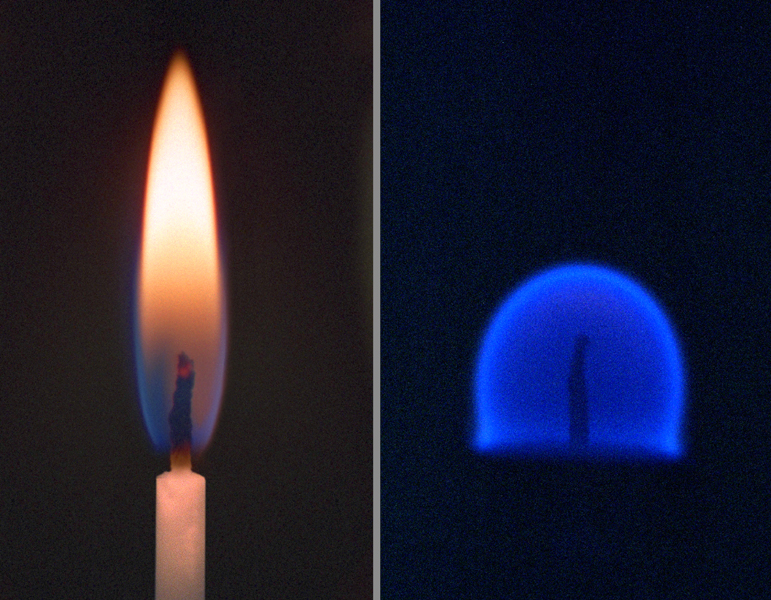
\includegraphics[scale=0.3]{P7}
\end{center}
Полум'я свічки при звичайних умовах та при невагомості \textit{(знімок з сайту NASA)}.\\

З іншого боку збільшення ваги внаслідок прискорення називають \textcolor{EdErablue}{\textbf{перевантаженням}}. Часто, наприклад, при виконанні трюків на літаках перевантаження вимірюють в кількості $g$. Наприклад, при польоті на спортивних літаках досягається перевантаження $10g$. Це означає, що вага при цьому $10mg$. 
\newpage

\subsubsection{Система тіл, що з'єднані ниткою}
Уявіть блок, що обертається. Через нього перекинута \textbf{нерозтяжна} нитка, на якій з двох сторін закріплені блоки різної маси $m_2 > m_1$. Таким чином з'явлається прискорення.
\begin{center}
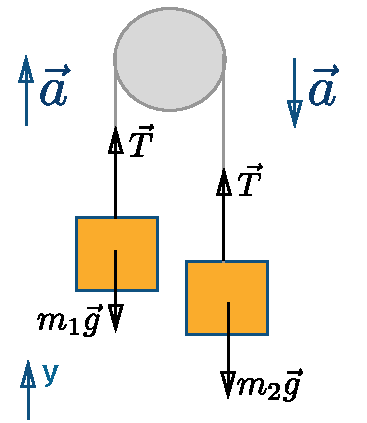
\includegraphics[scale=0.5]{P8}
\end{center}
Перше, що важливо. Якщо сказано, що нитка \textbf{нерозтяжна}, сила натягу $T$ у будь-якій її точці \textbf{однакова}. За третім законом Ньютона вага дорівнює силі натягу нитки. Виходить, що для даного випадку \textcolor{EdErablue}{\textbf{вага у двох тіл різної маси однакова}}. Це дуже важливий концептуальний момент. Не плутайте масу з вагою!\\

\hspace{-0.75cm} Другий момент. Коли ви маєте систему тіл, ви можете розглядати кожне тіло окремо. У англомовній літературі такий підхід називається \textcolor{EdErablue}{\textbf{Free body diagram}}.\\

Напрямимо вісь $y$ вгору та розглянемо кожне тіло окремо. 
\begin{center}
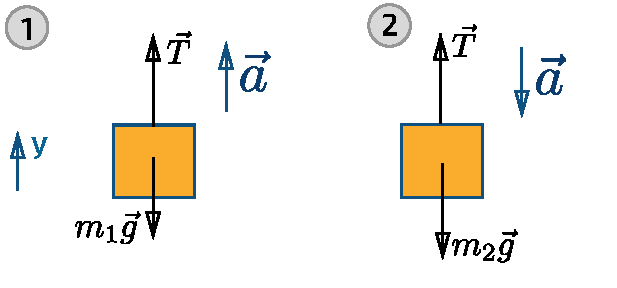
\includegraphics[scale=0.5]{P9}
\end{center}
\begin{itemize}
\item[1.] Другий закон Ньютона: $m_1\vec{g} + \vec{T} = m_1\vec{a}\,\,\Rightarrow\,\,-m_1g+T = m_1a$ $$T = m_1(a+g)$$
\item[2.] Другий закон Ньютона: $m_2\vec{g} + \vec{T} = m_2\vec{a}\,\,\Rightarrow\,\,-m_2g+T = -m_2a$ $$T = m_2(g-a)$$
\end{itemize}
Тепер можна прирівняти сили натягу нитки і отримати прискорення кожного з блоків. Вони, до речі, також однакові. $$m_1(a+g) = m_2(g-a)\,\,\Rightarrow\,\,a(m_1+m_2) = g(m_2-m_1)\,\,\Rightarrow\,\,\boxed{a = g\dfrac{m_2-m_1}{m_1+m_2}}$$ Оцінимо правильність формули. \begin{itemize} \item Якщо би \textcolor{EdErablue}{\textbf{маси були однакові}}, то система перебувала би у рівновазі.  $$m_1 = m_2 \rightarrow a= 0$$. \item Якщо би \textcolor{EdErablue}{\textbf{одного тіла взагалі не було}}, то інше тіло рухалось би просто з прискоренням $\vec{g}$. $$m_1 = 0 \rightarrow a = g\dfrac{m_2}{m_2} = g$$\end{itemize}
 
\section{Сила пружності та закон Гука}
Якщо прикласти силу до якогось тіла, то воно \textcolor{EdErablue}{\textbf{деформується}}. \\ \eoz{\textbf{Деформація} – це зміна форми твердого тіла під дією зовнішньої сили.\\ \newline
\textbf{Пружна деформація} – деформація, яка повністю зникає після припинення дії зовнішньої сили. Форма тіла повертається у своє "звичне" \thinspace положення. } 

\begin{multicols}{2}
\vspace{-0.4cm}
\begin{center}
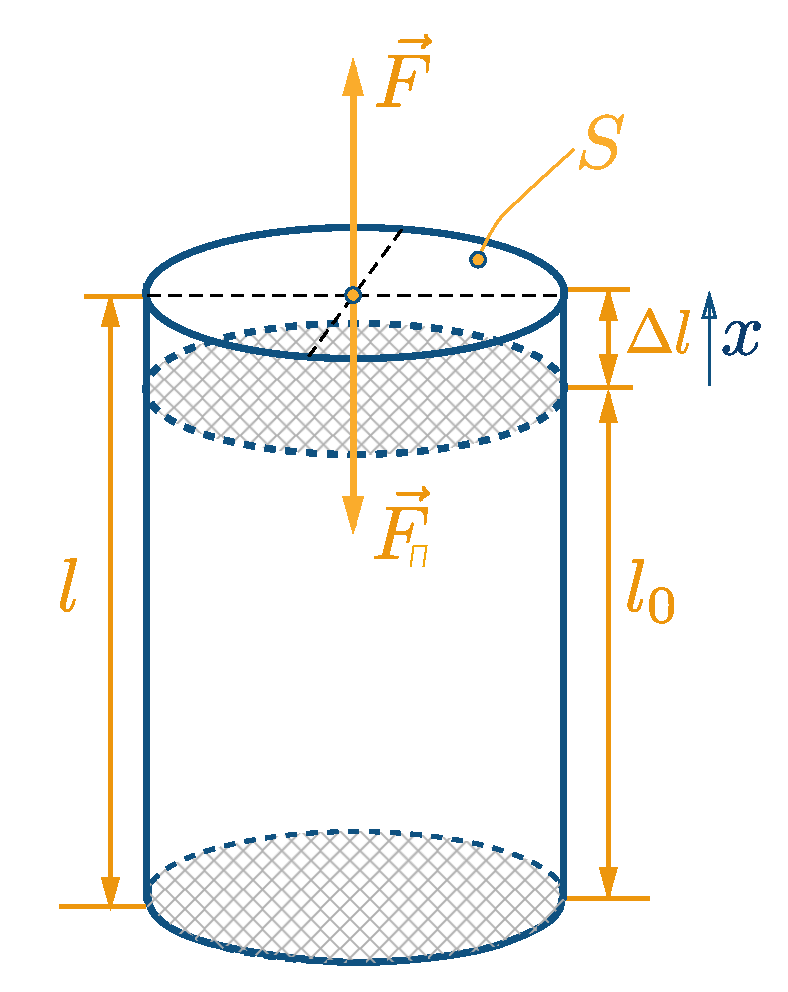
\includegraphics[scale=0.3]{P10}
\end{center}
\columnbreak

\begin{flushleft}
\textcolor{white}{.}\\
\textcolor{white}{.}\\
\textcolor{white}{.}\\
$l_0$ – довжина тіла у спокої;\\
$l$ - довжина тіла після деформації;\\
$\Delta l = l-l_0$ – видовження тіла;\\
$S$ – площа поперечного перерізу;\\
$\vec{F}$ –  прикладена сила;\\
$\vec{F}_{\text{П}}$ – сила пружності;
\end{flushleft}
\end{multicols}

\eoz{\textbf{Сила пружності $\vec{F}_{\text{П}}$} – сила, що виникає внаслідок деформації тіла і напрямлена в протилежну сторону до напрямку, вздовж якого відбувається деформація. }

На рисунку зображено тверде тіло, яке розтягують з силою $\vec{F}$. Виникає сила пружності $\vec{F}_{\text{П}}$, яка противиться деформації тіла і намагається повернути його в "звич-\\ний" \thinspace стан. \\

\begin{center}
\textcolor{EdErablue}{\textbf{Інтуітивно зрозумілі наступні моменти}}
\end{center}

\begin{itemize} \item[1.] Чим більша початкова довжина $l_0$, тим легше видовжити тіло на певну $\Delta l$ $$\Delta l \sim l_0$$  \item[2.]Чим більше прикладена сила $\vec{F}$, тим більше видовження тіла $\Delta l$ $$\Delta l \sim F$$ \item[3.]Чим більша площа  перерізу $S$, тим складніше видовжити тіло на певну $\Delta l$ $$\Delta l \sim \dfrac{1}{S}$$\end{itemize}

\textcolor{EdErablue}{\textbf{З усього вищезазначеного: $\boxed{\Delta l \sim \dfrac{Fl_0}{S}}$}}\\

Перетворивши отриману пропорційність отримаємо $\dfrac{F}{S} \sim \dfrac{\Delta l}{l_0}$\\

Ми використали усі параметри, що пов'язані з формою об'єкта. Залишилось для повної рівності використати параметр, який характеризує фізичну властивість матеріала створювати спротив диформації – \textcolor{EdErablue}{\textbf{модуль Юнга $E$ }}[$\dfrac{H}{\text{м}^2} = \text{Паскаль (Па)}$].\\ 
\begin{center}
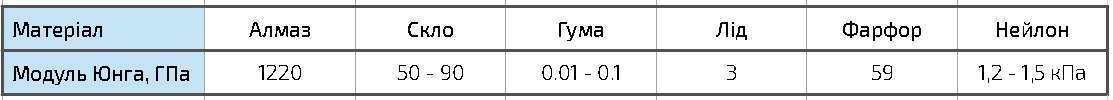
\includegraphics[scale=0.8]{P18}
\end{center}

Тепер ми готові к отриманню фундаментального закону, який пов'язує силу \newline пружності з видовженням тіла:
\begin{center}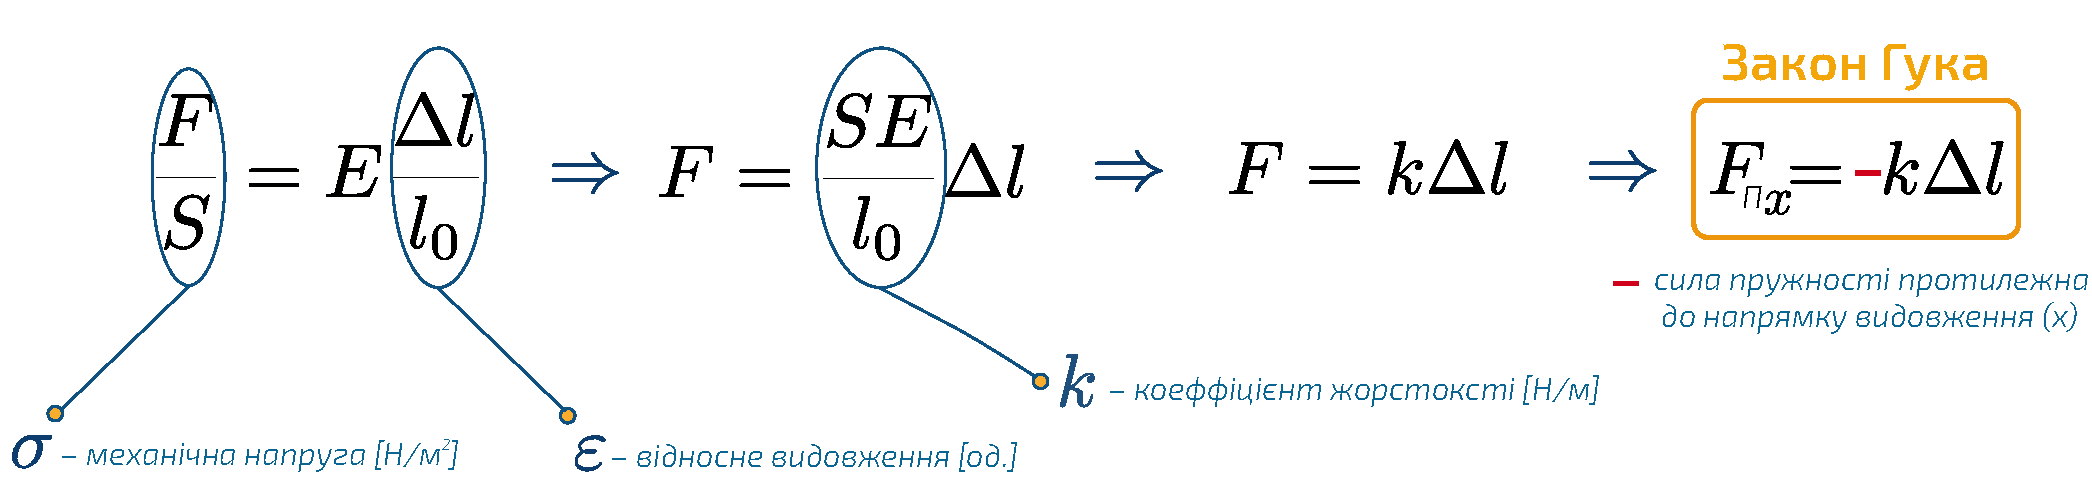
\includegraphics[scale=0.46]{P14} \end{center}
Закон Гука говорить про пропорційність між силою пружності $F_{\text{П}}$, яка виникає внаслідок деформації і видовженням тіла $\Delta l$. Чим більший коефіцієнт жорсткості $k$, тим швидше зі збільшенням видовження зростає сила пружності, яка намагається повернути тіло у свій "звичний" \thinspace стан. На рисунку $k = tg\,\alpha$.
\begin{center}
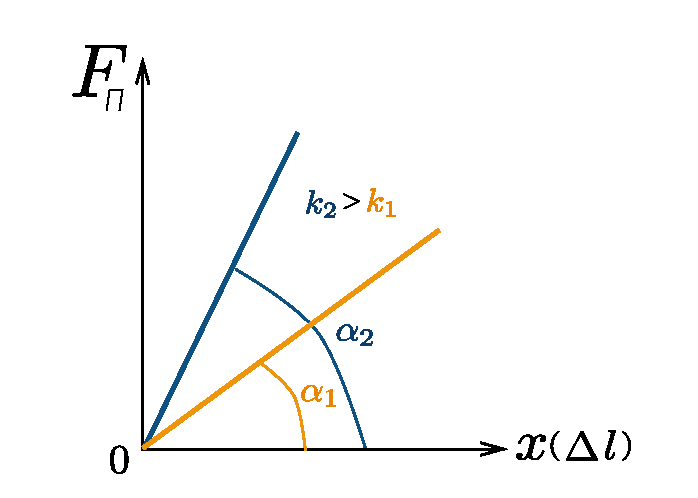
\includegraphics[scale=0.6]{P13}
\end{center}
Слід зауважити, що закон Гука в реальному житті виконується до \textbf{певної межі} по механічній напрузі. Після цієї межі тіло вже стає деформованим і не повертається у початковий стан. В школі не розглядається цей випадок. 

\newpage
\subsection{Послідовне та паралельне з'єднання пружин}
В задачах з пружинами використовується закон Гука. При цьому на відміну від розглянутої нами деформації твердих тіл, тут використовується саме коефіцієнт жорстоксті $k$. На рисунку зображено видовження пружини під дією сили $\vec{F}$ та виникаючу внаслідок цього силу $\vec{F}_{\text{П}}$, напрямлену протилежно до напрямку здійснення видовження (x).
\begin{center}
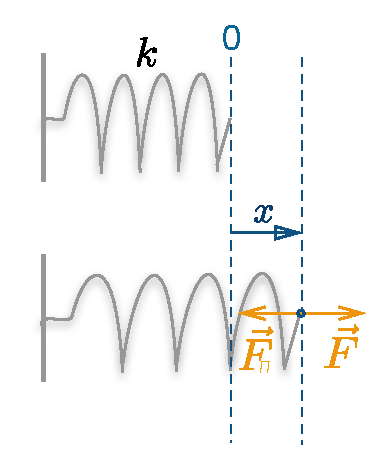
\includegraphics[scale=0.6]{P15}
\end{center}
Комбінація пружин з різними коефіцієнтами жорсткості $k_1, k_2...k_n$ може бути заміненою однією еквівалентною пружиною з певним $k$. Для того, щоб вміти робити такі операції розглянемо паралельне та послідовне з'єднання пружин. 
\begin{itemize}
\item[\textbf{\textcolor{EdErablue}{1.}}] \textcolor{EdErablue}{\textbf{Паралельне з'єднання пружин}} 
Нехай дві пружини з $k_1$ та $k_2$ з'єднані паралельно. Тоді, якщо ми закріпимо вантаж, як зображено на рисунку, то внаслідок дії сили тяжіння $\vec{F}_{T}$ виникає деформація пружин і відповідно дві сили пружності $\vec{F}_1$ і $\vec{F}_2$.
\begin{center}
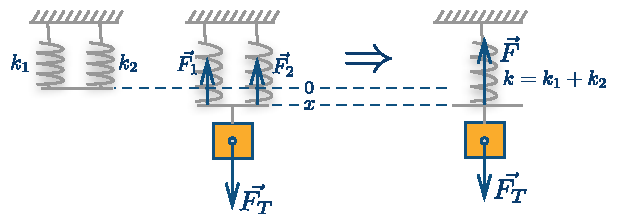
\includegraphics[scale=1]{P16}
\end{center}
Модуль сили пружності першої пружини: $F_1 = k_1x$\\
Модуль сили пружності другої пружини: $F_2 = k_2x$\\
За другим законом Ньютона: $\vec{F}_{T} + \vec{F}_1 + \vec{F}_2 = 0\,\,\Rightarrow \,\, F_T = F_1 + F_2$ \textcolor{EdErablue}{$$F_T = k_1x + k_2x$$}
Коли ми замінемо цю систему однією еквівалентною пружиною з коефіцієнтом жорсткості $k$, то сила пружності, яка в ній виникне буде дорівнювати силі тяжіння: \textcolor{EdErablue}{$ F = F_T = kx$}\\ 
Отже, якщо пружини з'єднані паралельно, то їх можна замінити однією пружиною, коефіцієнт жорсткості якої є сумою коефіцієнтів кожної із пружин: $$kx = k_1x + k_2x\,\,\Rightarrow\,\,\boxed{k=k_1+k_2}$$
\newpage
\item[\textbf{\textcolor{EdErablue}{2.}}] \textcolor{EdErablue}{\textbf{Послідовне з'єднання пружин}} 
Нехай дві пружини з $k_1$ та $k_2$ з'єднані послідовно. Тоді, якщо ми закріпимо вантаж, як зображено на рисунку, то внаслідок дії сили тяжіння $\vec{F}_{T}$ виникає деформація пружин і відповідно  сила пружності ${F}$ в кожній з пружин. Це зрозуміло, якщо використати третій закон Ньютона. Сила тяжіння викликає силу пружності у першій пружині, яка дорівнює силі тяжіння. З такою ж силою перша пружина діє на другу, і в ній виникає сила пружності, яка також дорівнює силі тяжіння. $F_1 = F_2 = F$ 
\begin{center}
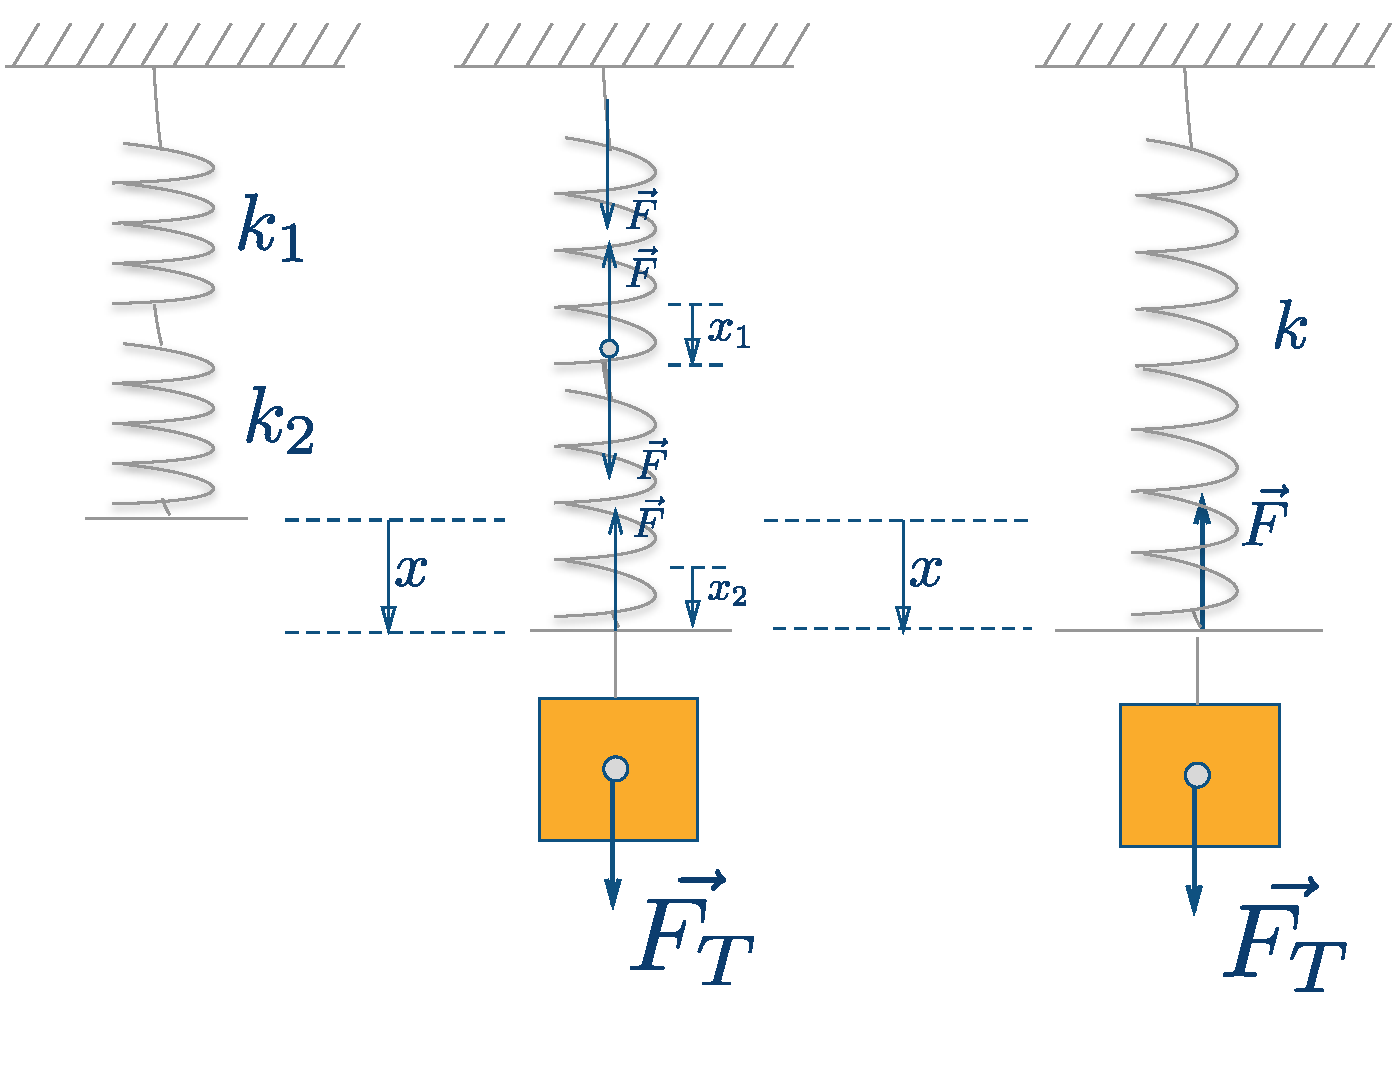
\includegraphics[scale=0.35]{P17}
\end{center}
Кожна пружина внаслідок дії на них однакової сили розтягується на різні $x_1$ та $x_2$. Якщо ми систему послідовно з'єднаних пружин замінимо однією еквівалент-\\ною, то видовження такої пружини $x$ повинно дорівнювати сумі видовжень $x_1$ та $x_2$. Давайте отримаємо для кожної з пружин видовження та підставимо у $x = x_1 + x_2$.\\

Видовження першої пружини: $x_1 = \dfrac{F}{k_1}$\\
Видовження другої пружини: $x_2 = \dfrac{F}{k_2}$\\
Видовження еквівалентної пружнии: $x = \dfrac{F}{k}$\\

Підставляємо у $x = x_1 + x_2$: $$\dfrac{F}{k} = \dfrac{F}{k_1}+ \dfrac{F}{k_2}\,\,\Rightarrow \,\, \boxed{\dfrac{1}{k} = \dfrac{1}{k_1} + \dfrac{1}{k_2}}$$
Отже, якщо пружини з'єднані послідовно, то їх можна замінити однією пружиною, коефіцієнт жорсткості якої можна розрахувати за допомогою вищезазначеної формули. 
\end{itemize}

\end{document}

